%%% LaTeX Template: Article/Thesis/etc. with colored headings and special fonts
%%%
%%% Source: http://www.howtotex.com/
%%% Feel free to distribute this template, but please keep to referal to http://www.howtotex.com/ here.
%%% February 2011
%%%
%%% Modified October 2015 by CDM

%%% Preamble
\documentclass[11pt,letterpaper]{article}
\usepackage[margin=1.0in]{geometry}
\usepackage[T1]{fontenc}
\usepackage[bitstream-charter]{mathdesign}
\usepackage[latin1]{inputenc}					
\usepackage{amsmath}						
\usepackage{xcolor}
\usepackage{cite}
\usepackage{hyphenat}
\usepackage{graphicx}
\usepackage{float}
\usepackage{subfigure}
\usepackage{sectsty}
\usepackage[compact]{titlesec} 
\usepackage[tablegrid]{vhistory}
\allsectionsfont{\color{accentcolor}\scshape\selectfont}

\usepackage{titlesec}
\setcounter{secnumdepth}{4}

%%% Definitions
\definecolor{accentcolor}{rgb}{0.0,0.0,0.5} 
\newcommand{\teamname}{Project Iris}
\newcommand{\productname}{Iris}
\newcommand{\coursename}{CSE 4316: Senior Design I}
\newcommand{\semester}{Summer 2016}
\newcommand{\docname}{System Requirements Specification}
\newcommand{\department}{Department of Computer Science \& Engineering}
\newcommand{\university}{The University of Texas at Arlington}
\newcommand{\authors}{Neil Simmons \\ Tyler D'Spain \\ Matthew Zielke \\ Syed Uddin \\ Tony McDonald}


%%% Headers and footers
\usepackage{fancyhdr}
	\pagestyle{fancy}						% Enabling the custom headers/footers
\usepackage{lastpage}	
	% Header (empty)
	\lhead{}
	\chead{}
	\rhead{}
	% Footer
	\lfoot{\footnotesize \teamname \ - \semester}
	\cfoot{}
	\rfoot{\footnotesize page \thepage\ of \pageref{LastPage}}	% "Page 1 of 2"
	\renewcommand{\headrulewidth}{0.0pt}
	\renewcommand{\footrulewidth}{0.4pt}

%%% Change the abstract environment
\usepackage[runin]{abstract}			% runin option for a run-in title
%\setlength\absleftindent{30pt}			% left margin
%\setlength\absrightindent{30pt}		% right margin
\abslabeldelim{\quad}	
\setlength{\abstitleskip}{-10pt}
\renewcommand{\abstractname}{}
\renewcommand{\abstracttextfont}{\color{accentcolor} \small \slshape}	% slanted text

\titleformat{\paragraph}
{\normalfont\normalsize\color{accentcolor}\bfseries}{\theparagraph}{1em}{}
\titlespacing*{\paragraph}
{0pt}{3.25ex plus 1ex minus .2ex}{1.5ex plus .2ex}

%%% Start of the document
\begin{document}

%%% Cover sheet
{\centering \huge \color{accentcolor} \sc \textbf{\department \\ \university} \par}
\vspace{1 in}
{\centering \huge \color{accentcolor} \sc \textbf{\docname \\ \coursename \\ \semester} \par}
\vspace{0.5 in}
\begin{figure}[h!]
	\centering
   	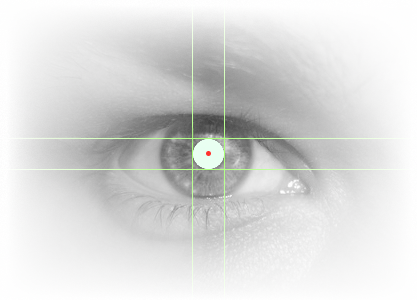
\includegraphics[width=0.60\textwidth]{images/project-iris}
\end{figure}
\vspace{0.5 in}
{\centering \huge \color{accentcolor} \sc \textbf{\teamname \\ \productname} \par}
\vspace{0.5 in}
{\centering \large \sc \textbf{\authors} \par}
\newpage


%\vspace{1 in}
%\centerline{January 13th, 2012}
%\newpage

%%% Revision History
\begin{versionhistory}
  	\vhEntry{0.1}{07.29.2016}{NS\textbackslash{}TD\textbackslash{}MZ\textbackslash{}SU\textbackslash{}TM}{document creation}
  	\vhEntry{0.2}{10.02.2016}{NS}{Update to new information}
\end{versionhistory}
\newpage

%%% Table of contents
\setcounter{tocdepth}{2}
\tableofcontents
\newpage

%%% List of figures and tables (optional)
\listoffigures
%\listoftables
\newpage

\section{Product Concept}
Project Iris is a software solution that will work in conjunction with an Intel RealSense SR300 camera to provide 3D gaze tracking information to a host computer. Ultimately the target for this solution are developers looking to incorporate 3D gaze tracking into their existing applications, or develop new applications around the added functionality Project Iris can provide. Project Iris will be open source and provided via a GitHub repository to any developer who wishes to use it.

\subsection{Purpose and Use}
Project Iris will provide 3D gaze tracking information to a host computer in the form of x and y coordinates similar to the way an operating system might provide mouse coordinates to a program. To accommodate this Project Iris will also provide a calibration utility and a screen overlay to indicate where the user is currently looking. This is to be used in conjunction with other software which is outside the scope of Project Iris, but could include mouse emulation, gaming, and efficiency/process improvements for desktop applications.

\subsection{Intended Audience}
Project Iris is not intended to be a standalone solution, but a tool developers of other software can include to create new and immersive user experiences. Game developers, application developers, and developers of accessibility software are all part of the target audience for Project Iris.

\begin{figure}[h!]
	\centering
   	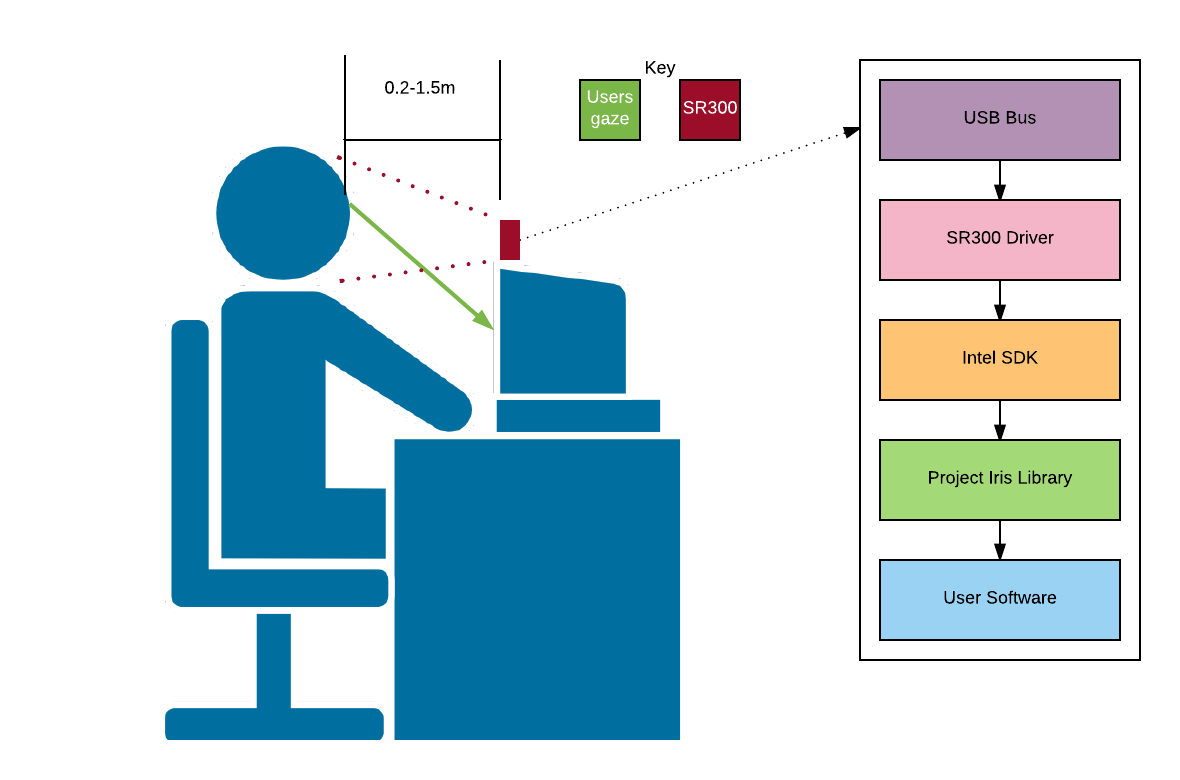
\includegraphics[width=0.60\textwidth]{images/project-iris-system-block}
    \caption{Project Iris system block diagram example}
\end{figure}

\newpage
\section{Product Description}
This section provides an overview of Project Iris, its components, and how it is intended to be used. The system will consist of an Intel RealSense SR300 camera, its driver and SDK software, and the open source code provided by Project Iris. The purpose of the system is to facilitate 3D gaze tracking for applications that do not currently have it, and to make it easier for applications in development to take advantage of 3D gaze tracking. 

\subsection{Features \& Functions}
The code provided by project Iris will include a calibration utility, an onscreen indicator of where the user is currently looking, and an API that will return the x and y coordinates of the user's current gaze position on the screen. Project Iris will be Open Source software intended for use on a Windows operating system and will require an Intel SR300.

\subsection{External Inputs \& Outputs}
Project Iris will work by using the data gathered from an Intel RealSense SR300 camera mounted as near the horizontal center and vertical top of a computer monitor as possible. The system will expect to be able to reconcile a user's eyes and facial landmarks from a distance of .2 - 1.5 meters. After a calibration procedure this data will be translated into x and y coordinates for use in other applications. In addition to the calibration utility and coordinate outputs via an API, the system will allow the developer to toggle on an indicator to visualize the current gaze position.

\subsection{Product Interfaces}
Project Iris will provide a calibration utility that will place a dot at different positions on the computer monitor (figure 2) and then use this data to output an estimate of the user's current gaze position relative to the screen. The position will be provided via an API call in the form of a pair of integers representing the estimated x and y coordinates of the user's gaze. In addition, the system will provide a toggle via the API to turn on a translucent dot that will allow for the visualization of the current estimated gaze position (figure 3).

\begin{figure}[h!]
	\centering
   	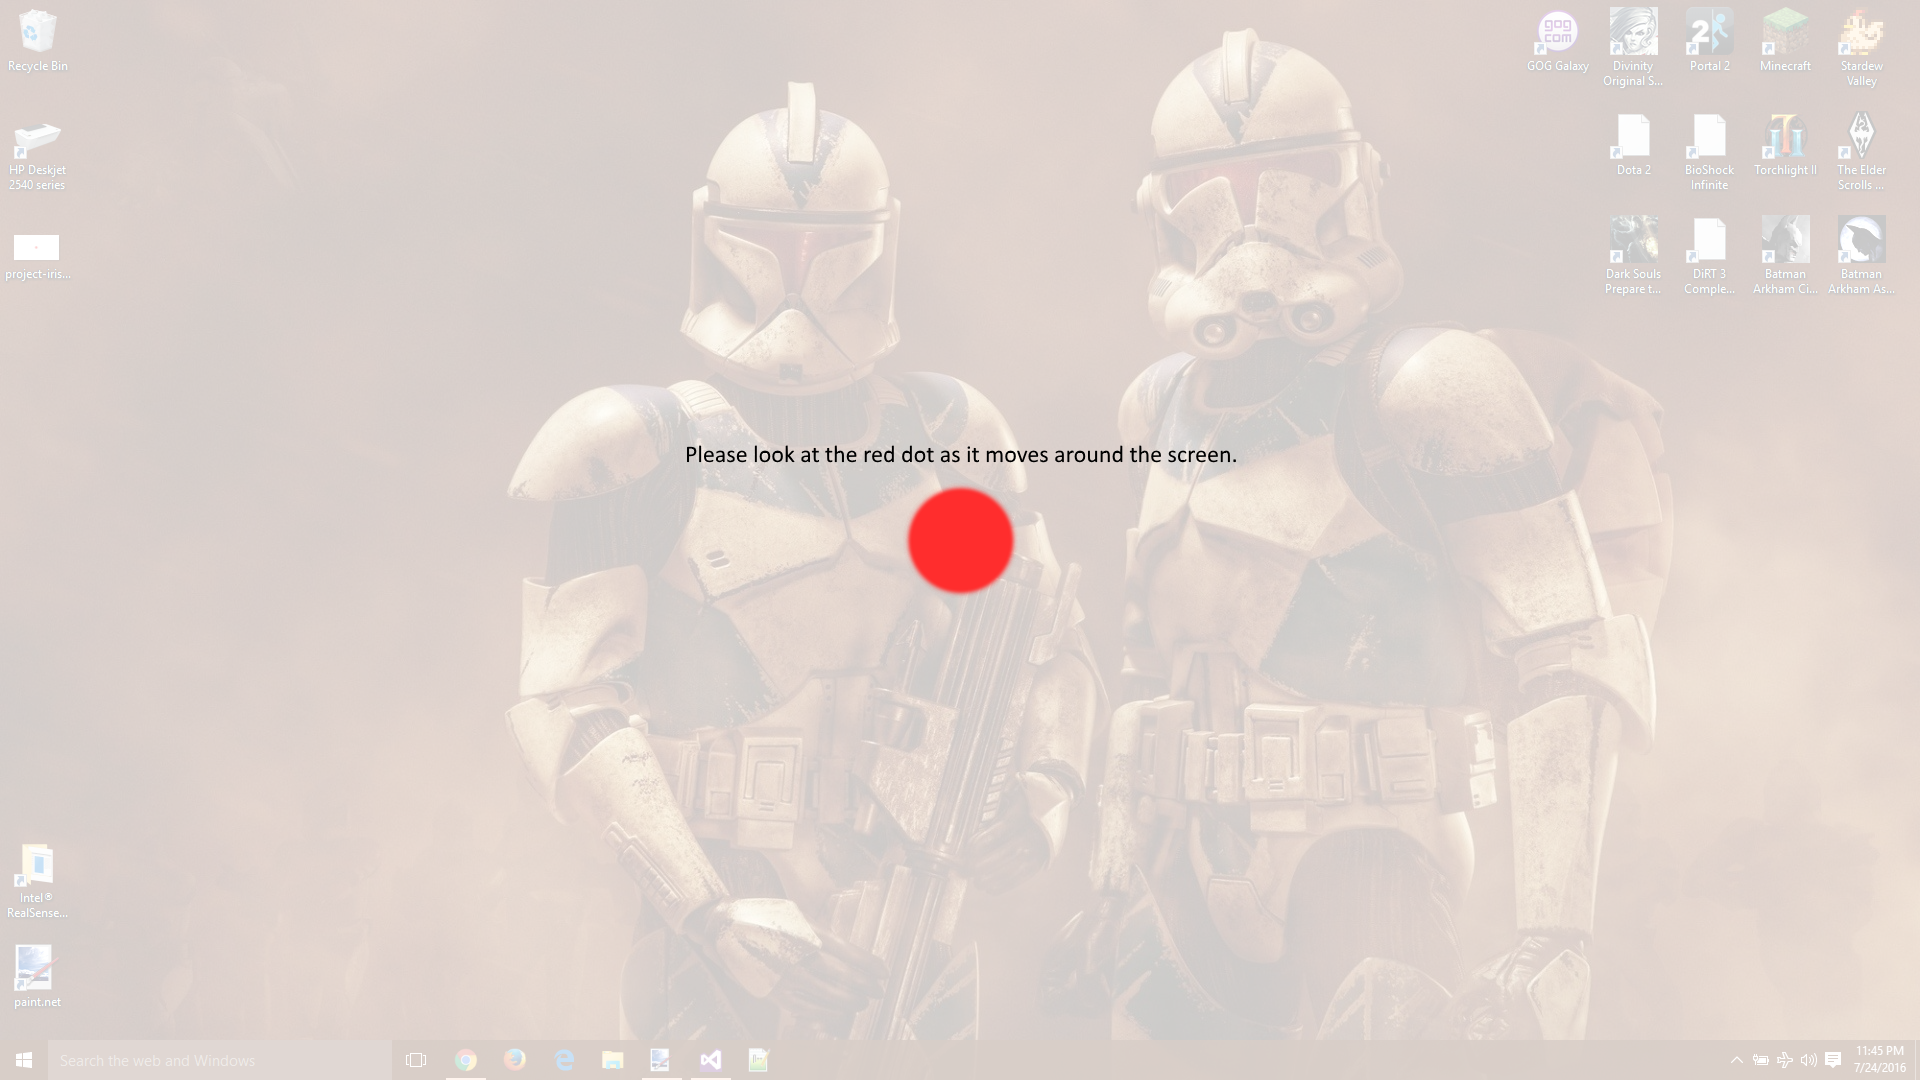
\includegraphics[width=0.60\textwidth]{images/project-iris-calibration}
    \caption{Calibration utility concept}
\end{figure}

\begin{figure}[h!]
	\centering
   	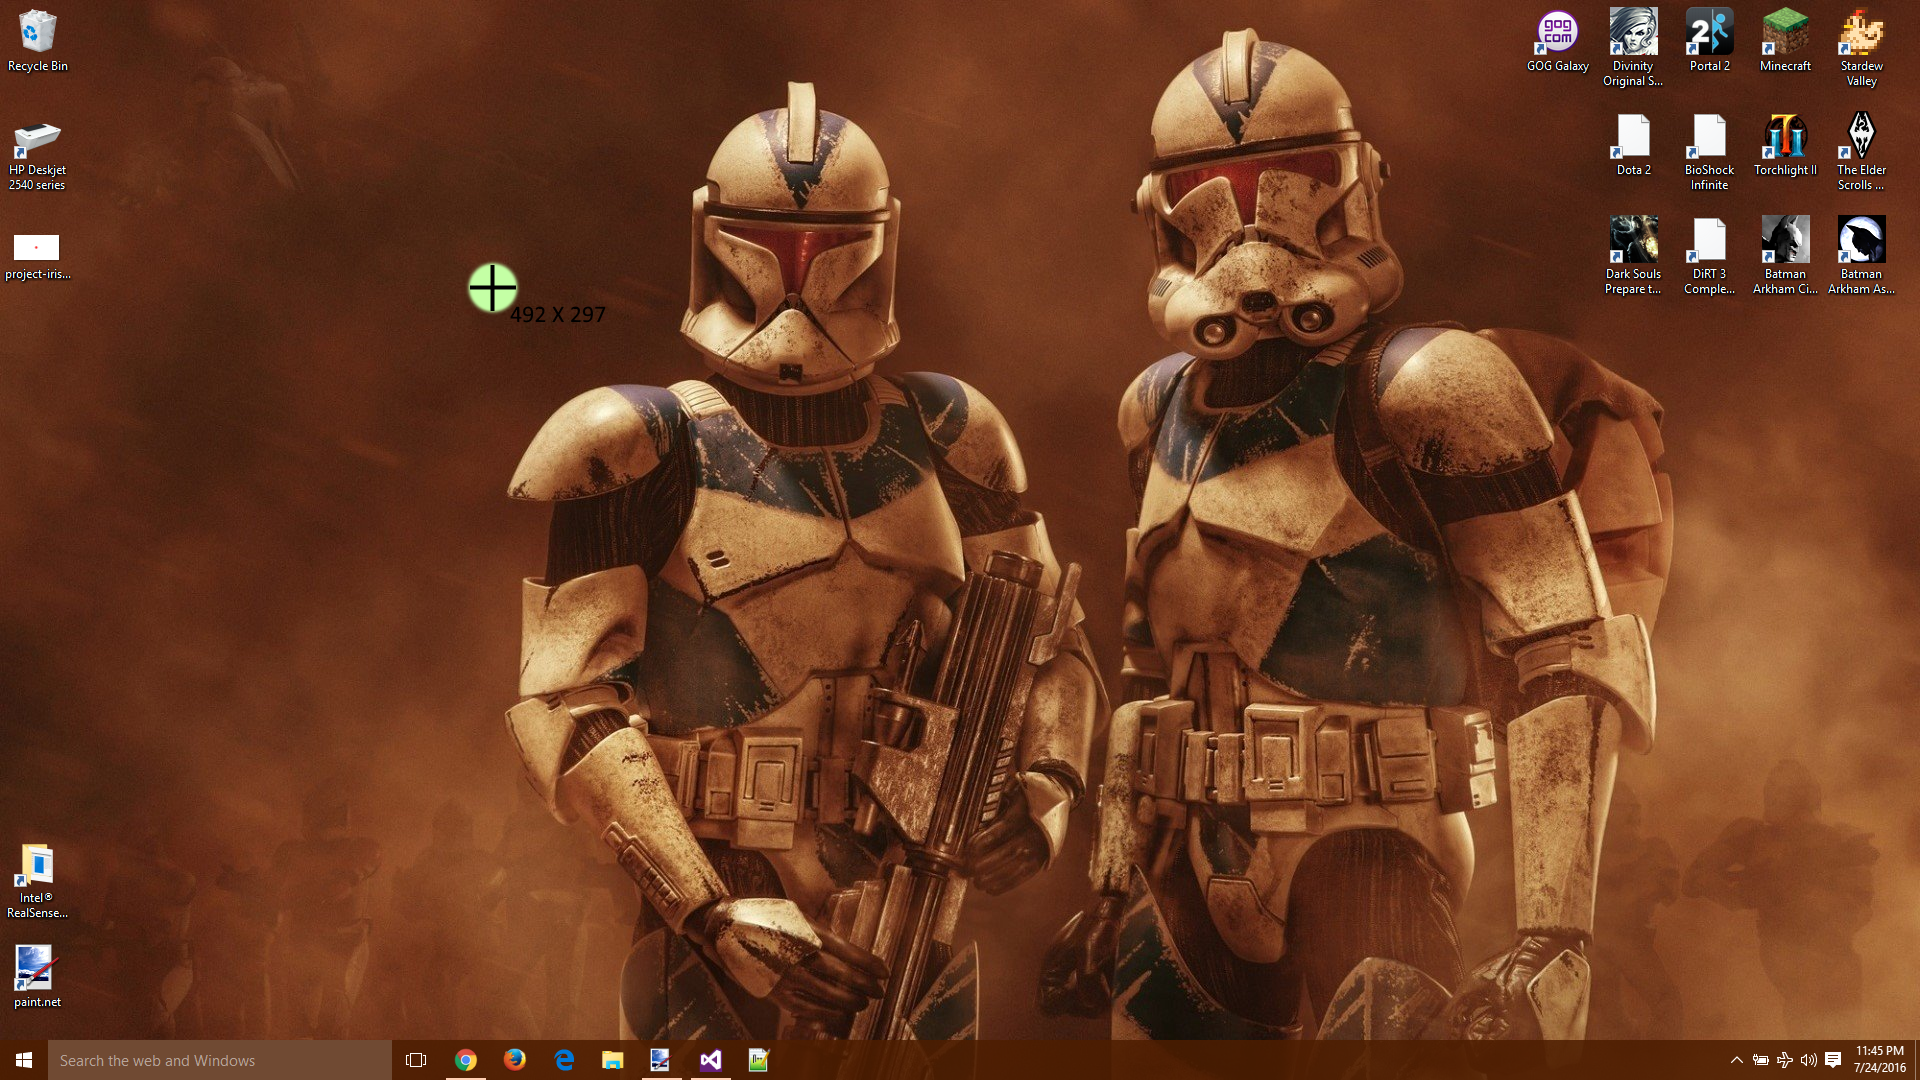
\includegraphics[width=0.60\textwidth]{images/project-iris-visualization}
    \caption{Visualization of the current gaze position concept}
\end{figure}
\newpage
\section{Customer Requirements}
Include a header paragraph specific to your product here. Customer requirements are those required features and functions specified for and by the intended audience for this product. This section establishes, clearly and concisely, the "look and feel" of the product, what each potential end-user should expect the product do and/or not do. Each requirement specified in this section is associated with a specific customer need that will be satisfied. In general Customer Requirements are the directly observable features and functions of the product that will be encountered by its users. Requirements specified in this section are created with, and must not be changed without, specific agreement of the intended customer/user/sponsor.

\subsection{Requirement Name}
\subsubsection{Description}
A detailed description of the feature/function that satisfies the requirement. For example: \textit{The box will be slate blue. This specific color is required in order to ensure that the box matches other similar boxes in the Box Systems Premium line of products. Slate blue is specified as \#007FFF, using six-digit hexadecimal color specification.} It is acceptable and advisable to include drawings/graphics in the description if it aids understanding of the requirement.
\subsubsection{Source}
The source of the requirement (e.g. customer, sponsor, specified team member (by name), federal regulation, local laws, CSE Senior Design project specifications, etc.)
\subsubsection{Constraints}
A detailed description of constraints on satisfying the requirement (e.g. one such constraint might be: \textit{The specified color must be commercially available in paint capable of adhering to the material of which the box is manufactured. (See customer requirement 3.x for production material specification.)}
\subsubsection{Standards}
A detailed description of any specific standards that apply to this requirement (e.g. \textit{NSTM standard xx.xxx.x. color specifications \cite{Rubin2012}}.)
\subsubsection{Priority}
The priority of this requirement relative to other specified requirements. Use the following priorities:
\begin{itemize}
\item Critical (must have or product is a failure)
\item High (very important to customer acceptance, desirability)
\item Moderate (should have for proper product functionality);
\item Low (nice to have, will include if time/resource permits)
\item Future (not feasible in this version of the product, but should be considered for a future release).
\end{itemize}

\subsection{Requirement Name}
\subsubsection{Description}
Detailed requirement description...
\subsubsection{Source}
Source
\subsubsection{Constraints}
Detailed description of applicable constraints...
\subsubsection{Standards}
List of applicable standards
\subsubsection{Priority}
Priority

\newpage
\section{Packaging Requirements}
This product shall be software only. There will be no hardware to deliver with Project Iris. As the camera used is packaged and shipped by a 3rd party. All software shall be located on Github as open source project.
\subsection{Source Code}
\subsubsection{Description}
The software source code shall be available on Github as an open source project. All source code shall be uploaded to Project Iris' repository on Github when completed.
\subsubsection{Source}
Team
\subsubsection{Priority}
High
\subsection{Binaries}
\subsubsection{Description}
Binaries shall be included on the Github repository as open source. Binary file(s) shall also be uploaded to Project Iris' repository on Github to make it easier for anyone to download and run with the right equipment.
\subsubsection{Source}
Team
\subsubsection{Priority}
Moderate
\subsection{Zip File}
\subsubsection{Description}
A zip file containing all project files shall also be included in the Github repository. A copy of all files including binaries shall be put into a zip file to make downloading easier and faster.
\subsubsection{Source}
Team
\subsubsection{Priority}
Moderate
\subsection{Intel Real Sense Camera}
\subsubsection{Description}
The RealSense camera shall be packaged and delivered by Intel. Since the software is developed for use with Intel's RealSense SR300 camera, the device is needed to run the software correctly. This device is packaged and shipped by Intel and we have no control over this.
\subsubsection{Source}
Team
\subsubsection{Priority}
Low
\newpage
%\section{Performance Requirements}
%Include a header paragraph specific to your product here. Performance requirements address items such as: how fast specific critical operations must complete; how long it takes to start/stop activities; how long the battery must last; maximum time it must take to set up; etc.

\subsection{Requirement Name}
\subsubsection{Description}
Detailed requirement description...
\subsubsection{Source}
Source
\subsubsection{Constraints}
Detailed description of applicable constraints...
\subsubsection{Standards}
List of applicable standards
\subsubsection{Priority}
Priority
%\newpage
\section{Safety Requirements}
Safety is a priority for Project Iris therefore it shall be safe for all users.  The Intel SR300 RealSense camera will be used and is considered to be completely safe for extended use with the human eye.  
\subsection{Laser}
\subsubsection{Description}
The device shall be a Class 1 laser product  so that the maximum permissible exposure to the naked eye cannot be exceeded.
\subsubsection{Source}
OSHA 
\subsubsection{Standards}
The device must be a Class 1 Laser project
\subsubsection{Priority}
High
\subsection{Power Source}
\subsubsection{Description}
The devices power source shall be safe and sufficient. The device shall use USB 3.0 technology for connectivity as well as a power source.  This technology eliminates the hazard of dealing with additional power supplies and power outlets while providing sufficient power to the device.
\subsubsection{Source}
Intel 
\subsubsection{Priority}
Low
\subsection{Weight and Size}
\subsubsection{Description}
The Devices dimensions shall be light and compact in order for it to be able to be able to mounted onto any display screen.  Be it a lightweight laptop or heavier monitor.
\subsubsection{Source}
Team
\subsubsection{Priority}
Low
\newpage
\section{Maintenance \& Support Requirements}
Include a header paragraph specific to your product here. Maintenance and support requirements address items specific to the ongoing maintenance and support of your product after delivery. Think of these requirements as if you were the ones who would be responsible for caring for customers/end user after the product is delivered in its final form and in use "in the field". What would you require to do this job? Specify items such as: where, how and who must be able to maintain the product to correct errors, hardware failures, etc.; required support/troubleshooting manuals/guides; availability/documentation of source code; related technical documentation that must be available for maintainers; specific/unique tools required for maintenance; specific software/environment required for maintenance; etc.

\subsection{Requirement Name}
\subsubsection{Description}
Detailed requirement description...
\subsubsection{Source}
Source
\subsubsection{Constraints}
Detailed description of applicable constraints...
\subsubsection{Standards}
List of applicable standards
\subsubsection{Priority}
Priority
\newpage
\section{Other Requirements}
There are Some additional requirements that the hardware need in order for the system to work.  These requirements are specific to the Intel SR300 SDK. 

\subsection{Processor}
\subsubsection{Description}
Computers using the SR300 shall be equipped with a 6th generation Intel processor.  With the SR300 being a developer's kit by intel, it requires the use of an intel processors.  Moreover, it requires the use of a 6th generation or better processor.
\subsubsection{Source}
Intel
\subsubsection{Priority}
High
\subsection{Graphics Processor}
\subsubsection{Description}
Computers using the SR300 shall have a graphics card with OpenCL 1.2.  Another requirement that the SR300 has is that you must have a computer equipped with a graphics card that supports OpenCL 1.2.  That means that you must have a fairly new graphics card in order for the camera to work with your computer.
\subsubsection{Source}
Intel
\subsubsection{Priority}
High
\subsection{Connection Interface}
\subsubsection{Description}
Computers using the SR300 shall be equipped with a USB 3.0 connection interface.  The SR300 uses USB 3.0.  Any USB version prior to this will not power the camera therefore it will not work.
\subsubsection{Source}
Intel
\subsubsection{Priority}
High
\subsection{Operating System}
\subsubsection{Description}
Computers using the SR300 must be equipped with Microsoft Windows 10. The OS requirement for the SR300 is Microsoft Windows 10.  Without this OS the camera cannot be used.
\subsubsection{Source}
Intel
\subsubsection{Priority}
High
\newpage
\section{Future Items}
In this last section, you will reiterate all requirements that are listed as priority 5. This is repetitive, but necessary as a concise statement of features/functions that were considered/discussed and documented herein, but will NOT be addressed in the prototype version of the product due to constraints of budget, time, skills, technology, feasibility analysis, etc. Use the following format for this section.

\subsection{Requirement Name}
\subsubsection{Description}
Detailed requirement description...
\subsubsection{Source}
Source
\subsubsection{Constraints}
Detailed description of applicable constraints...
\subsubsection{Standards}
List of applicable standards
\subsubsection{Priority}
Priority
\newpage

%%% References
\bibliographystyle{plain}
\bibliographystyle{reference/IEEEtran_custom}
\bibliography{reference/refs}{}

\end{document}